\section{Problem 2}
\textit{Using the FDTD matlab code given at the course, design a Yagi-Uda antenna that has a gain of at least 6 dBi at 850 Mhz.}\\

We followed the design proposal for a Yagi-Uda antenna originally proposed by Hidetsugu Yagi in \cite{lit:YAGI}. The specific details for a three elements is found from the standardization from the National Bureau of Standards (US) shown in \tref{tab:Yagi-jpg}.

\begin{figure}[!h]
  \centering
  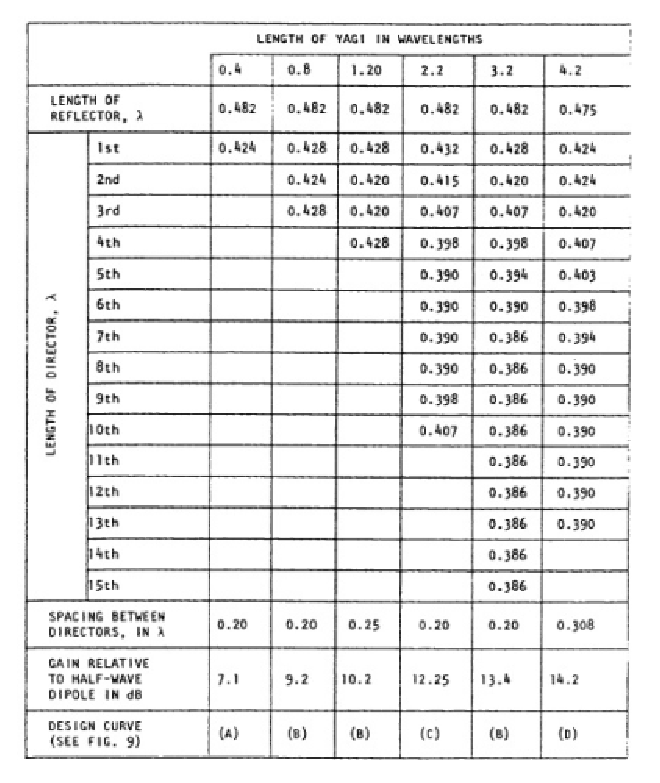
\includegraphics[width=10cm]{Yagi-jpg.eps}
  \caption{Table showing the length needed for optimized gain @400MHz. Reflector is placed $0.2\lambda$ behind the driven element \cite[p.~7]{lit:NBS}}
  \label{tab:Yagi-jpg}
\end{figure}

Since the antenna should have a required gain of 6 dBi at 850 Mhz, our wavelength of interest is $\lambda = \SI{0.353}{\meter}$. Given that wavelength, since we wanted to have an accurate FDTD simulation, we set the cell size to $\SI{0.01}{\meter}$. The literature recommends to use a cell size of at least a tenth of a wavelength, with the chosen value we were sure that we were fulfilling that requirement.\\

The simulation geometry is shown in the \figref{fig:3_element_yagi-uda_geometry} and the simulation parameters are shown in \tref{tab:antenna_param}

\begin{figure}[!h]
  \centering
  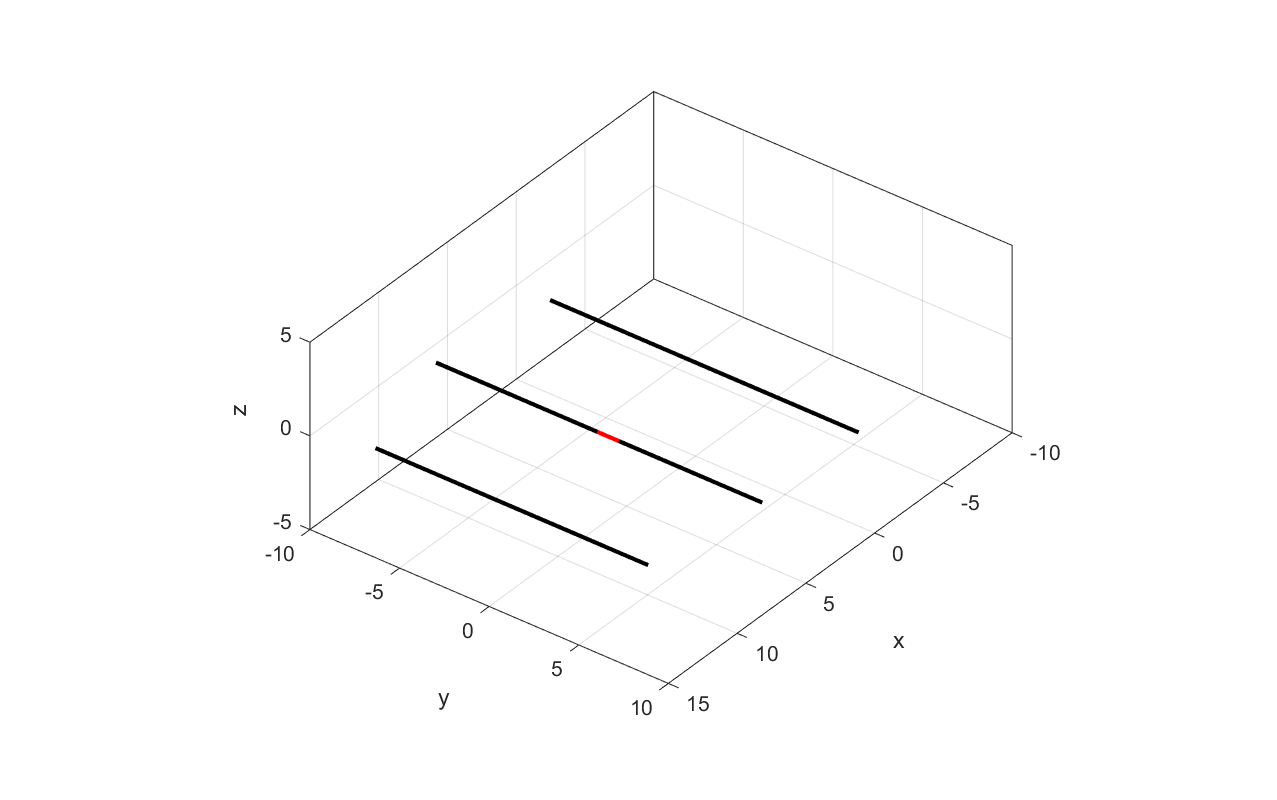
\includegraphics[width=12cm]{3_element_yagi-uda_geometry.eps}
  \caption{Figure showing the angles involved in the dipole inclination and rotation}
  \label{fig:3_element_yagi-uda_geometry}
\end{figure}

\ptable{| p{12cm} | p{6cm} |}{ %
Parameter 		&	Value 			\\ \hline
Reflector size 		        &	$17 cells$	$\approx$ 170mm        \\ \hline
Dipole size 		        &	$18 cells$	$\approx$ 176mm        \\ \hline
Director size 		        &	$15 cells$	$\approx$ 150mm        \\ \hline
Reflector position (x axis) 		        &	$0 cells$	        \\ \hline
Dipole position (x axis) 		        &	$7 cells$	        \\ \hline
Director position (x axis) 		        &	$14 cells$	        \\ \hline
Cell size 		        &	$\SI{0.01}{\meter}$	        \\ \hline
Excitation lower freq 		        &	$\SI{1}{\hertz}$	        \\ \hline
Excitation higher freq 		        &	$\SI{1.7}{\giga\hertz}$	        \\ \hline
}{Simulation and design parameters}{tab:antenna_param}

The design Yagi antenna is giving a gain patten as shown in \figref{fig:3_element_yagi-uda_pol_pattern} we can see that the three elements Yagi-Uda antenna presents a gain of 8.9dBi. These results are fairly close to those found in the reference shown in \tref{tab:Yagi-jpg} where it is stated that the gain of a 3-elements Yagi-Uda antenna is expected to be of 7.1 dBi. Finding the resulting gain in the polar plot is not that easy. Therefore the Cartesian version is also presented in \figref{fig:3_element_yagi-uda_cart_pattern}. This plot can be compared to the reference plot shown in \figref{fig:Yagi_CardPlot}. The matching of the antenna is a bit off but as seen in \figref{fig:3_element_yagi-uda_s11}. However it was not a part of the exercise to match the antenna so this is not optimized. 

\begin{figure}[!h]
  \centering
  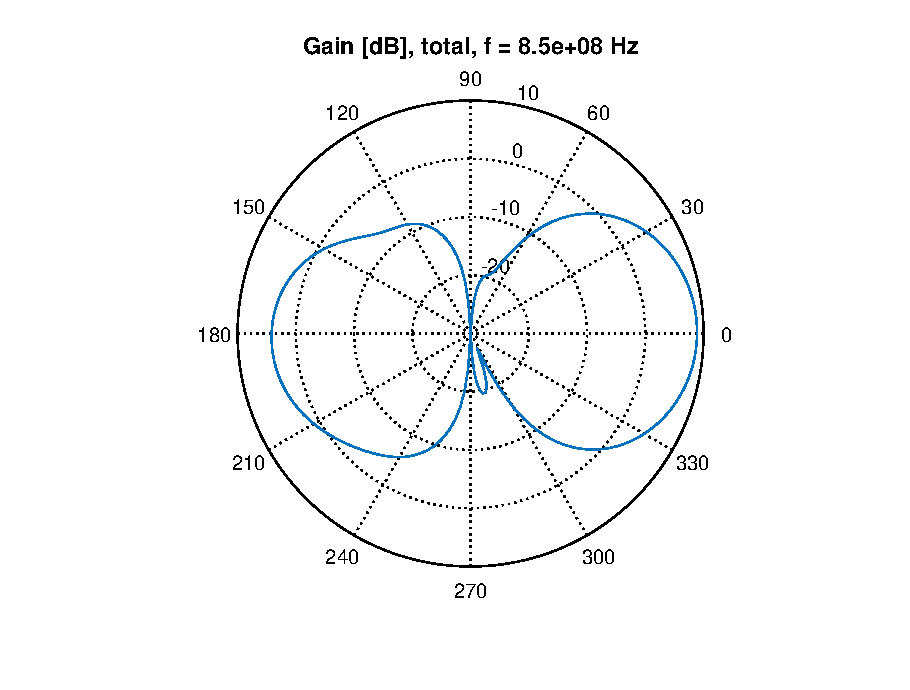
\includegraphics[width=11cm]{3_element_yagi-uda_pol_pattern.eps}
  \caption{Figure showing the polar gain patten of the designed antenna.}
  \label{fig:3_element_yagi-uda_pol_pattern}
\end{figure}

\begin{figure}[!h]
  \centering
  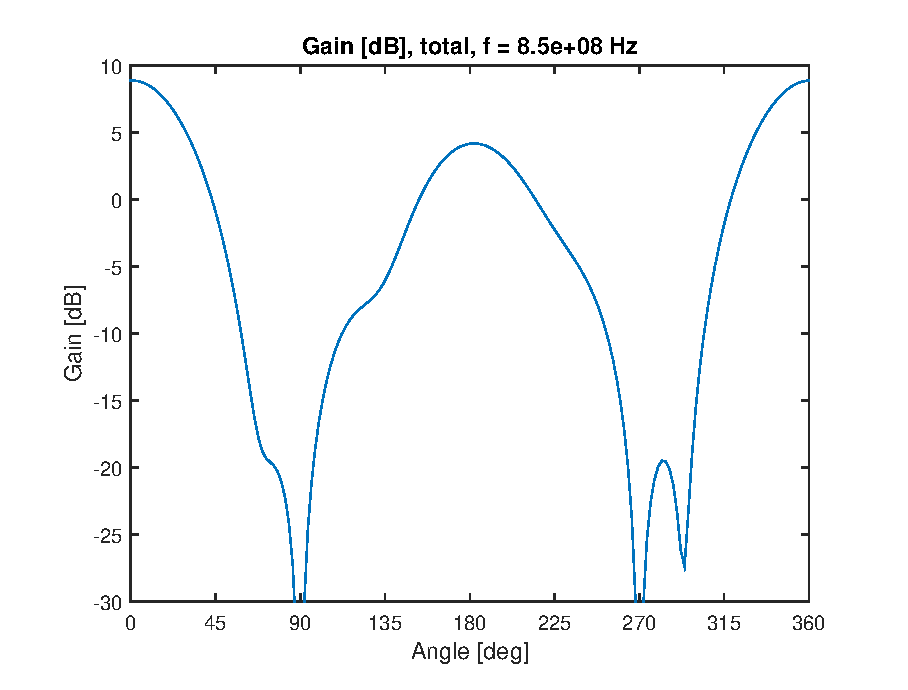
\includegraphics[width=11cm]{3_element_yagi-uda_cart_pattern.eps}
  \caption{Figure showing the Cartesian gain patten for the designed antenna.}
  \label{fig:3_element_yagi-uda_cart_pattern}
\end{figure}

\begin{figure}[!h]
  \centering
  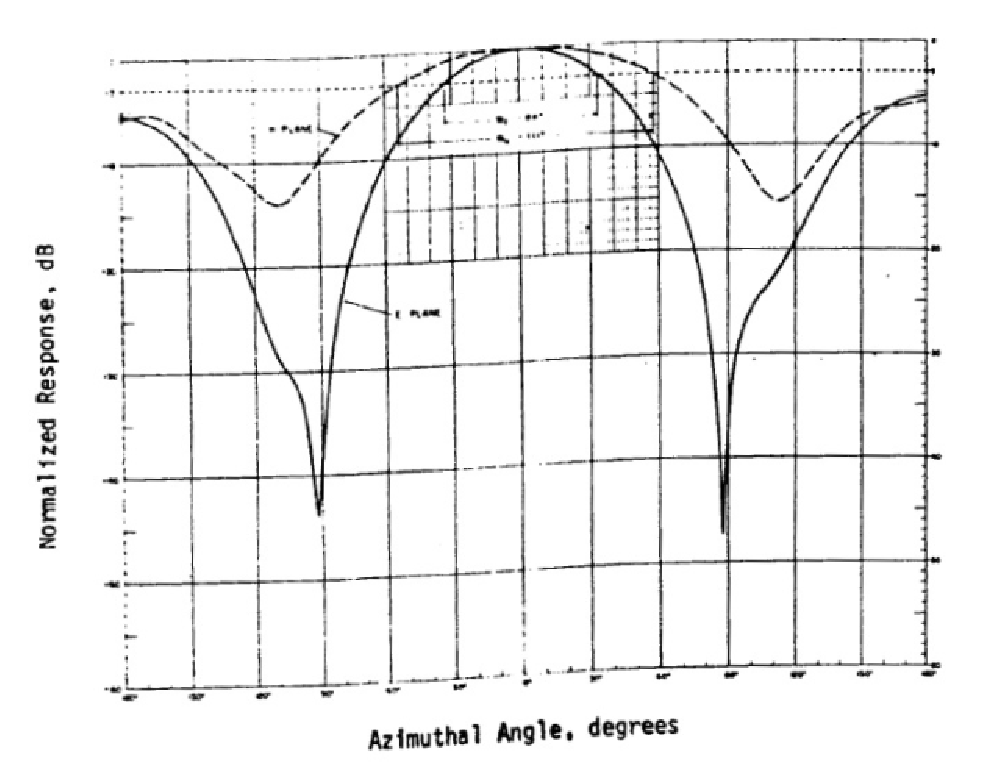
\includegraphics[width=11cm]{Yagi_CardPlot.eps}
  \caption{Figure showing the Cartesian gain patten for the reference antenna \cite[p.~12]{lit:NBS}.}
  \label{fig:Yagi_CardPlot}
\end{figure}

\begin{figure}[!h]
  \centering
  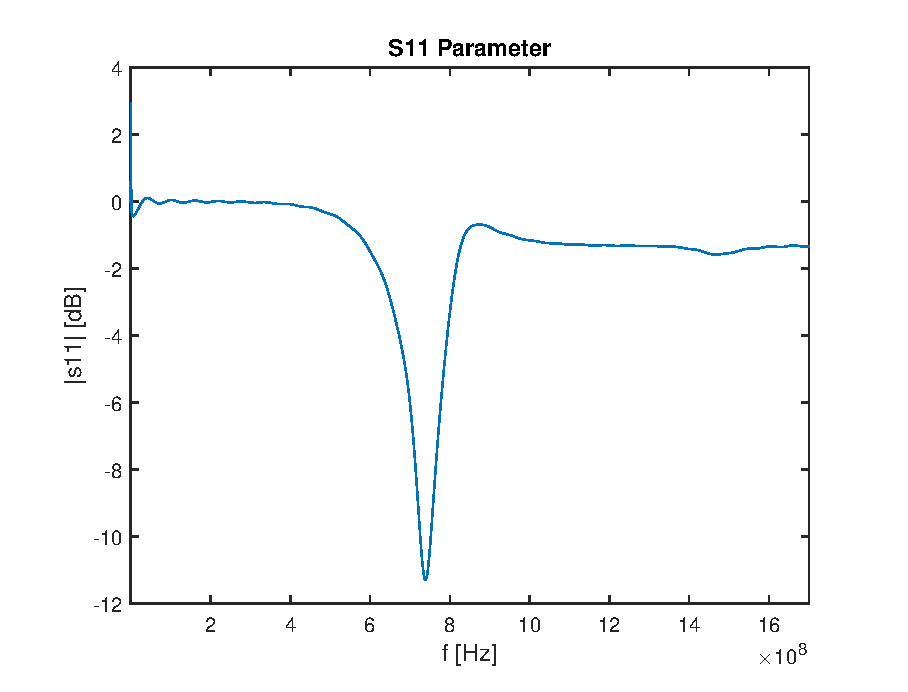
\includegraphics[width=11cm]{3_element_yagi-uda_s11.eps}
  \caption{Figure showing the s11/matching of the antenna}
  \label{fig:3_element_yagi-uda_s11}
\end{figure}
\FloatBarrier

From the plots we can see that the designed antenna indeed give a good gain in the intended direction. However we also have a large back-lobe which for many applications is not wanted. We have tried to optimize the design resulting in the following design parameters. The polar gain patten is shown in \figref{fig:3_element_yagi-uda_pol_pattern_2}.

\ptable{| p{12cm} | p{6cm} |}{ %
Parameter 		&	Value 			\\ \hline
Reflector size 		        &	$18 cells$	        \\ \hline
Dipole size 		        &	$16 cells$	        \\ \hline
Director size 		        &	$12 cells$	        \\ \hline
Reflector position (x axis) 		        &	$0 cells$	        \\ \hline
Dipole position (x axis) 		        &	$9 cells$	        \\ \hline
Director position (x axis) 		        &	$14 cells$	        \\ \hline
Cell size 		        &	$\SI{0.01}{\meter}$	        \\ \hline
Excitation lower freq 		        &	$\SI{1}{\hertz}$	        \\ \hline
Excitation higher freq 		        &	$\SI{1.7}{\giga\hertz}$	        \\ \hline
}{Simulation and design parameters for optimized antenna}{tab:antenna_param_2}

\begin{figure}[!h]
  \centering
  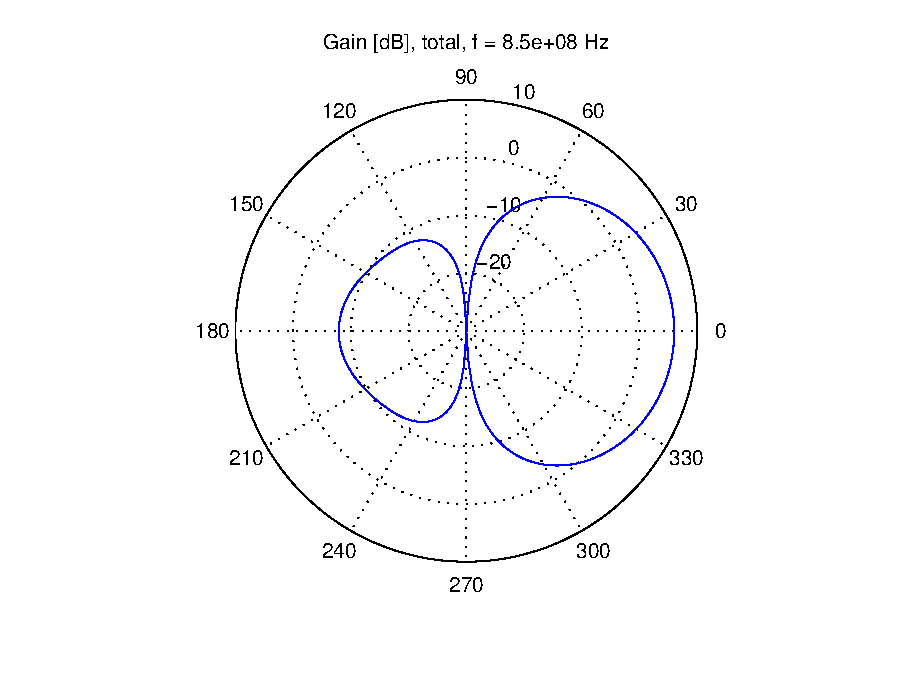
\includegraphics[width=12cm]{yagi_radiation_pattern_director.eps}
  \caption{Figure showing the polar gain patten of the optimized designed antenna.}
  \label{fig:3_element_yagi-uda_pol_pattern_2}
\end{figure}
\FloatBarrier

As it can be seen here in \figref{fig:3_element_yagi-uda_pol_pattern_2} this antenna have a smaller back-lobe as the reflector is slightly larger that the wavelength giving that it will reflect more of the power. The price to pay for this is in the gain in the wanted direction which is now only 6.1 dBi as the beam with is also larger in this design.